\subsection{Website fingerprinting}

\subsubsection{Preliminaries}
The adversary considers a set of webpages that we call \emph{DNS
Analyzed Webpages (DAW)}. Note that this set might be different from the
set of monitored/unmonitored webpages that the adversary collected
traffic traces on the ingress side for.
For each webpage the adversary observes which domains are requested by
the browser when loading the webpage. The set of domains requested,
their order, uniqueness, how stable they are over several repetitions of
loading the webpage, and what TTL they have, comprises the
\emph{Webpage DNS Fingerprint (WDF)} of the webpage.
The adversary constructs a dataset that maps each webpage in the DAW set
to its WDF.

\subsubsection{The DAW dataset}
We build our DAW dataset by using Tor Browser Bundle (TBB) 5.5.4
configured to not browse over Tor: TBB ensures that the browser behavior is
identical to a TBB user over Tor, and by not using Tor we bypass IP-blacklists
and CAPTCHAs triggered by IP-addresses of Tor-exits \cite{Khattak2016a}.
During week 16 in 2016 we browsed Alexa top one million websites from a
university network in Sweden, collecting five samples from each website.
Collection was done in rounds, where each round uniformly randomly browsed all one
million websites before visiting the same website again.

Table~\ref{tab:dns-censor} shows the percentage of websites in our dataset that
risks censorship by CloudFlare or Akami if collecting data over Tor, as
identified by Khattak et al.~\cite{Khattak2016a}. We also include Google, which
reportedly restricts access to Tor users (when searching), due to
their prevalance in the dataset.
% Only TODO websites are free of CloudFlare, Akamai and Google.

We collected in total 2,540,941 distinct domain names over 60,828,453 DNS requests.
There are 2,260,534 \emph {unique domains} that are only requested on a
particular website. Figure~\ref{fig:unique-domains} shows the percentage of sites
with unique domains for different parts of Alexa top one million.
For 96.8\% of all sites there exists at least one uniqe domain, and the more popular
a site is the less likely it is to have a unique domain.

Table~\ref{tab:daw-ttls} -- TTLs in entire data set, raw and adjusted for Tor,
also for unique domains.

\begin{figure}[t]
	\centering
	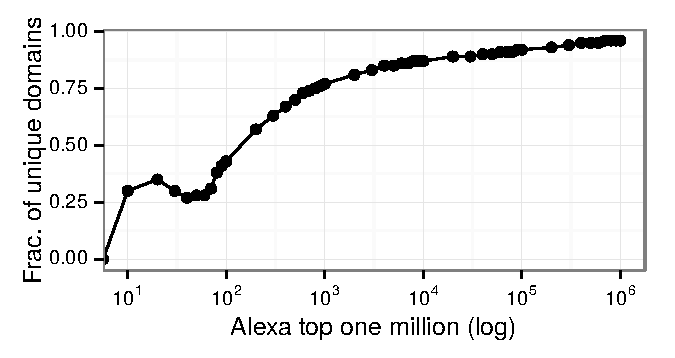
\includegraphics[width=\linewidth]{figures/dns-unique-domains.pdf}
	\caption{TODO: generate differently}
	\label{fig:unique-domains}
\end{figure}

\begin{table}[t]
	\centering
	\begin{tabular}{l r}
	\toprule
	\textbf{Description} & \textbf{Percentage} \\
	\midrule
	Website behind CloudFlare IP & 6.44 \\
	Domain on website uses CloudFlare & 25.81 \\
	Domain on website uses Akamai & 33.86 \\
	Domain on website uses Google & 77.43 \\
	\bottomrule
	\end{tabular}
	\caption{The percentage of websites on Alexa top-one-million using providers
	involved in censoring or restricting access to Tor~\cite{Khattak2016a}.}
	\label{tab:dns-censor}
\end{table}

\begin{table}[t]
	\centering
	\begin{tabular}{l c c c c}
	\toprule
	\textbf{DNS Requests} & \textbf{Median} & \textbf{Mean} & \textbf{Min} & \textbf{Max} \\
	\midrule
	per site & 10 & $12.2\pm11.2$ & 1 & 397 \\
	unique per site & 2 & $2.3\pm1.8$ & 0 & 363 \\
	\bottomrule
	\end{tabular}
	\caption{Statistics on the number of DNS requests.}
	\label{tab:daw-unique}
\end{table}


\begin{table}[t]
	\centering
	\begin{tabular}{l c c}
	\toprule
	\textbf{TTLs (s)} & \textbf{Median} & \textbf{Mean} \\
	\midrule
	% 2016/04/28 15:52:39 DNS records TTL mean 9780.0, std 42930.5, median 255.0, min 0.0, max 604800.0
	raw & 255 & $9780.0\pm42930.5$ \\ % & 0 & 604800 \\
	% 2016/04/28 15:44:05 DNS records TTL mean 701.5, std 755.3, median 255.0, min 60.0, max 1800.0
	Tor & 255 & $701.5\pm755.3$ \\ %& 60 & 1800 \\
	% 2016/04/28 15:52:39 	unique domain TTL mean 13022.2, std 35054.4, median 900.0, min 0.0, max 604800.0
	unique raw & 900 & $13022.2\pm35054.4$ \\ %& 0 & 604800 \\
	% 2016/04/28 15:44:05 	unique domain TTL mean 1005.3, std 789.6, median 900.0, min 60.0, max 1800.0
	unique Tor & 900 & $1005.3\pm789.6$ \\ %& 60 & 1800 \\
	% 2016/04/28 15:52:39 	unique domain _min_ TTL mean 3833.9, std 11073.6, median 60.0, min 0.0, max 604800.0
	min unique raw & 60 & $3833.9\pm11073.6$ \\ % & 0 & 604800 \\
	% 2016/04/28 15:44:05 	unique domain _min_ TTL mean 644.2, std 763.8, median 60.0, min 60.0, max 1800.0
	min unique Tor & 60 & $644.2\pm763.8$ \\ %& 60 & 1800 \\
	\bottomrule
	\end{tabular}
	\caption{%The TTL of DNS records observed in our DAW dataset.
	Raw TTLs are unprocessed while Tor TTLs adhere to Tor's TTL clipping.
	The unique prefix is for the TTL of unique domains while min unique only
	considers the unique domains with the minimum TTL for each website.}
	\label{tab:daw-ttls}
\end{table}

\subsubsection{Generating webpage DNS fingerprints}

\subsubsection{Enhancing WF attacks with DNS data}

% attack only one client
We take a client-centric view and assume that the adversary focuses on
one client to attack\footnote{This is a simplification and might
underestimate the adversary's power, because monitoring the traffic of
several users on the ingress-side is easily possible, for example when
the adversary operates one or more Tor entry guards.}.
%
% see several exits
We assume that the adversary observes DNS traffic from several exit
relays (either by operating a DNS resolver used by several exit relays,
or sniffing traffic from several exit relays to one or more DNS
resolvers).
%
% terminology observe/un-observed/client's exits
We distinguish between \emph{observed exits}, \ie~exit relays that use
DNS resolvers that are controlled or monitored by the adversary,
\emph{un-observed exits}, \ie~all exit relays except the observed exits,
and the \emph{client's exit}, \ie~the exit relay used by the client for
the current request.
%
% client's exit unknown
Note that the adversary does not know a priori which exit relay the
client uses, so the client's exit can be among the observed exits or the
un-observed exits.

%
We now describe how the adversary can use the data from the observed
exits to enhance website fingerprinting attacks.


\subsubsection{Egress DNS request analysis}

The adversary sees all DNS traffic of all observed exits, that is fully
qualified website domain names (not webpage URLs though), timestamped
and grouped per exit relay (\eg~labeled with the exit relay's IP
address).

When observing a new website request on the ingress side, that is a
traffic trace starting at time $t_0$, the adversary takes a
\emph{snapshot} of the continuously recorded DNS traffic data for each
observed exit relay. The snapshot from one exit relay is the set of
queries that were issued by this relay in the time-period from $t_0 - c$
to $t_0 + d$, where $c$ is the maximum TTL (30 min) and $d$ is the
maximum delay for DNS queries that can be caused by longer page load
times and Tor latency (probably one minute is enough?).

If the client's exit is among the observed exits, then all DNS queries
generated when loading the webpage (\ie~all domains in the webpage's
WDF) are included in the snapshot set from this exit. This is the case
because even if one domain name was already cached at the exit relay
(because this or another user of that exit visited the website before),
it must have been queried for during the last $c$ minutes, otherwise its
TTL would have expired and it would have been requested again (latest
$d$ minutes after the website request was issued).

The adversary can compare the snapshot sets of all observed exits with
the WDF of webpages in the DAW dataset in order to derive the
probability that a certain webpage was loaded by the client.

\begin{itemize}
  \item (per exit: note that we cannot take the union of all snapshot
		  sets ignoring exit labels, because the domains of a wepage's
		  WDF must all be found in one snapshot set. This is because one
		  page load happens from only one exit, so all DNS queries for
		  this page load will originate from the same exit relay)
  \item ordering: the webpages main domain must be requested first (but
		  order in snapshop set can be permuted due to cached other
		  requests for the same domain in different orders during the
		  last 30 minutes). For fresh domains (timestamps in the
		  snapshot set greater than $t_0$) require ordering as measured
		  (at least for first domain entry, maybe for more if
		  measurements show that order is robust over repetitions).
  \item weighting by cache-time and TTL information: assign lower weight
		  to domain entries in the snapshot set that have been cached
		  longer, take measured TTL into account (not only max tor
		  caching time)
  \item weighting by uniqueness: assign lower weight to domains in the
		  snapshot set that have lower uniqueness (\eg~
		  font.api.google.com should get a lower weight than
		  aftonbladet.se. Weight in range $[1..0]$, $1$ meaning that the
		  domain is unique in the DAW, $0$ meaning that the domain is
		  part of all WDFs in the DAW).
		  % weight(domain) = (|DAW| - count(domain)) / (|DAW| - 1)
\end{itemize}

We describe different approaches how an adversary could make use of the
snapshot sets to improve website fingerprinting.

\subsubsection{Two-classifier approach}

The analysis of the DNS data as described above can be considered to be
a separate website fingerprinting classifier. This classifier is build
using the DAW dataset. It takes the continuous recordings of all
observed DNS requests and a point in time $t_0$ as input. It then
constructs the snapshot sets for each exit and outputs a probability
distribution $D_{egress}$, describing the probability for each webpage
in the DAW that the client visited this webpage.
%
Using state of the art, classical website fingerprinting techniques on
the traffic trace observed on the ingress side (\eg~cite Panchenko et
al., Hayes et al. and Wang?), the adversary can obtain a probability
distribution $D_{ingress}$, describing the probability for each webpage
in the monitored set that the client visited this webpage.
%
So when the adversary observes a new webpage request from the client (to
delineate between browsing sessions is a difficult task, though, say
\cite{Coull2007a}), she uses a classical WF classifier to obtain
$D_{ingress}$ from the observed traffic trace on the ingress side. At
the same time, she uses the DNS data observed at the egress side to
obtain $D_{egress}$. Finally the adversary combines the two
distributions and outputs the webpage with the highest probability in
the resulting joint distribution.
%
When combining $D_{ingress}$ and $D_{egress}$, the adversary can take
knowledge about the accuracy of the classifiers into account, \eg~weight
the $D_{ingress}$ distribution higher if the classical WF is more
reliable then the DNS data analysis.
%
Classical WF techniques have high recall but only mediocre precision.
The DNS data provides very high precision if the client's exit is among
the observed exits and most of the WDF have unique domain sets (refer to
uniqueness statistic here when analysis is done). So a combination of
the two could result in a technique with both high recall and high
precision.


\subsubsection{Close-the-world approach}

Another approach is to use the DNS data to inform the construction of
the training set for a classical WF classifier.
%
If the adversary happens to observe the client's exit, then the game
changes to a closed-world setting because the adversary knows that the
client must have visited one of the webpages whose WDF is compatible
with one of the snapshot sets.
%
We say that a webpage is \emph{compatible} with a snapshot set, if all
domains that are requested when loading the wepage (\ie~all domains
contained in the WDF of the wepage) have corresponding entries in that
snapshot set. We say that a webpage is compatible with the set of all
snapshot sets, or simply ``with the snapshot sets'', from all observed
exits, if it is compatible with at least one of them. 
%
The adversary cannot know though, if she observes the client's exit. 
%
To account for this, the adversary can first apply a classifier that is
only trained on those webpages that are compatible with the snapshot
sets, then apply a classifier which is trained on a standard set of
training instances, and then combine their outputs.
%
Alternatively the adversary can extend a standard training set with a
higher number of training instances for all webpages that are compatible
with the snapshot sets.
%
Note that adapting the training set after the observation of a page load
is possible as the ingress trace can be recorded and first classified
after the classifier has been re-trained on the modified training set
(that was adapted to the egress DNS observations as described above).


\subsubsection{Simulating the snapshot Set}
(We want to estimate how much better WF becomes using DNS data. But we
are not 8.8.8.8 and don't have real data to do experiments. Therefore we
need to at least simulate the state of the snapshot sets at the time of
a page load.) %TODO
